\section{BigchainDB Transaction Latency}\label{sec:latency}

A key question is how long it takes for a transaction to get “etched in stone” (i.e. into a block that is \textsf{\textit{decided\_valid}}). 
To begin answering that question, we can trace the life of a transaction $\mathbf{t}$, from the time a client sends it to the time the client gets a confirmation that $\mathbf{t}$ is in a \textsf{\textit{decided\_valid}} block. 
Figure \ref{fig:bigchaindb_tx_life_1} and Figure \ref{fig:bigchaindb_tx_life_2} illustrate the life of a transaction.

\begin{figure}[!ht]
  \centering
  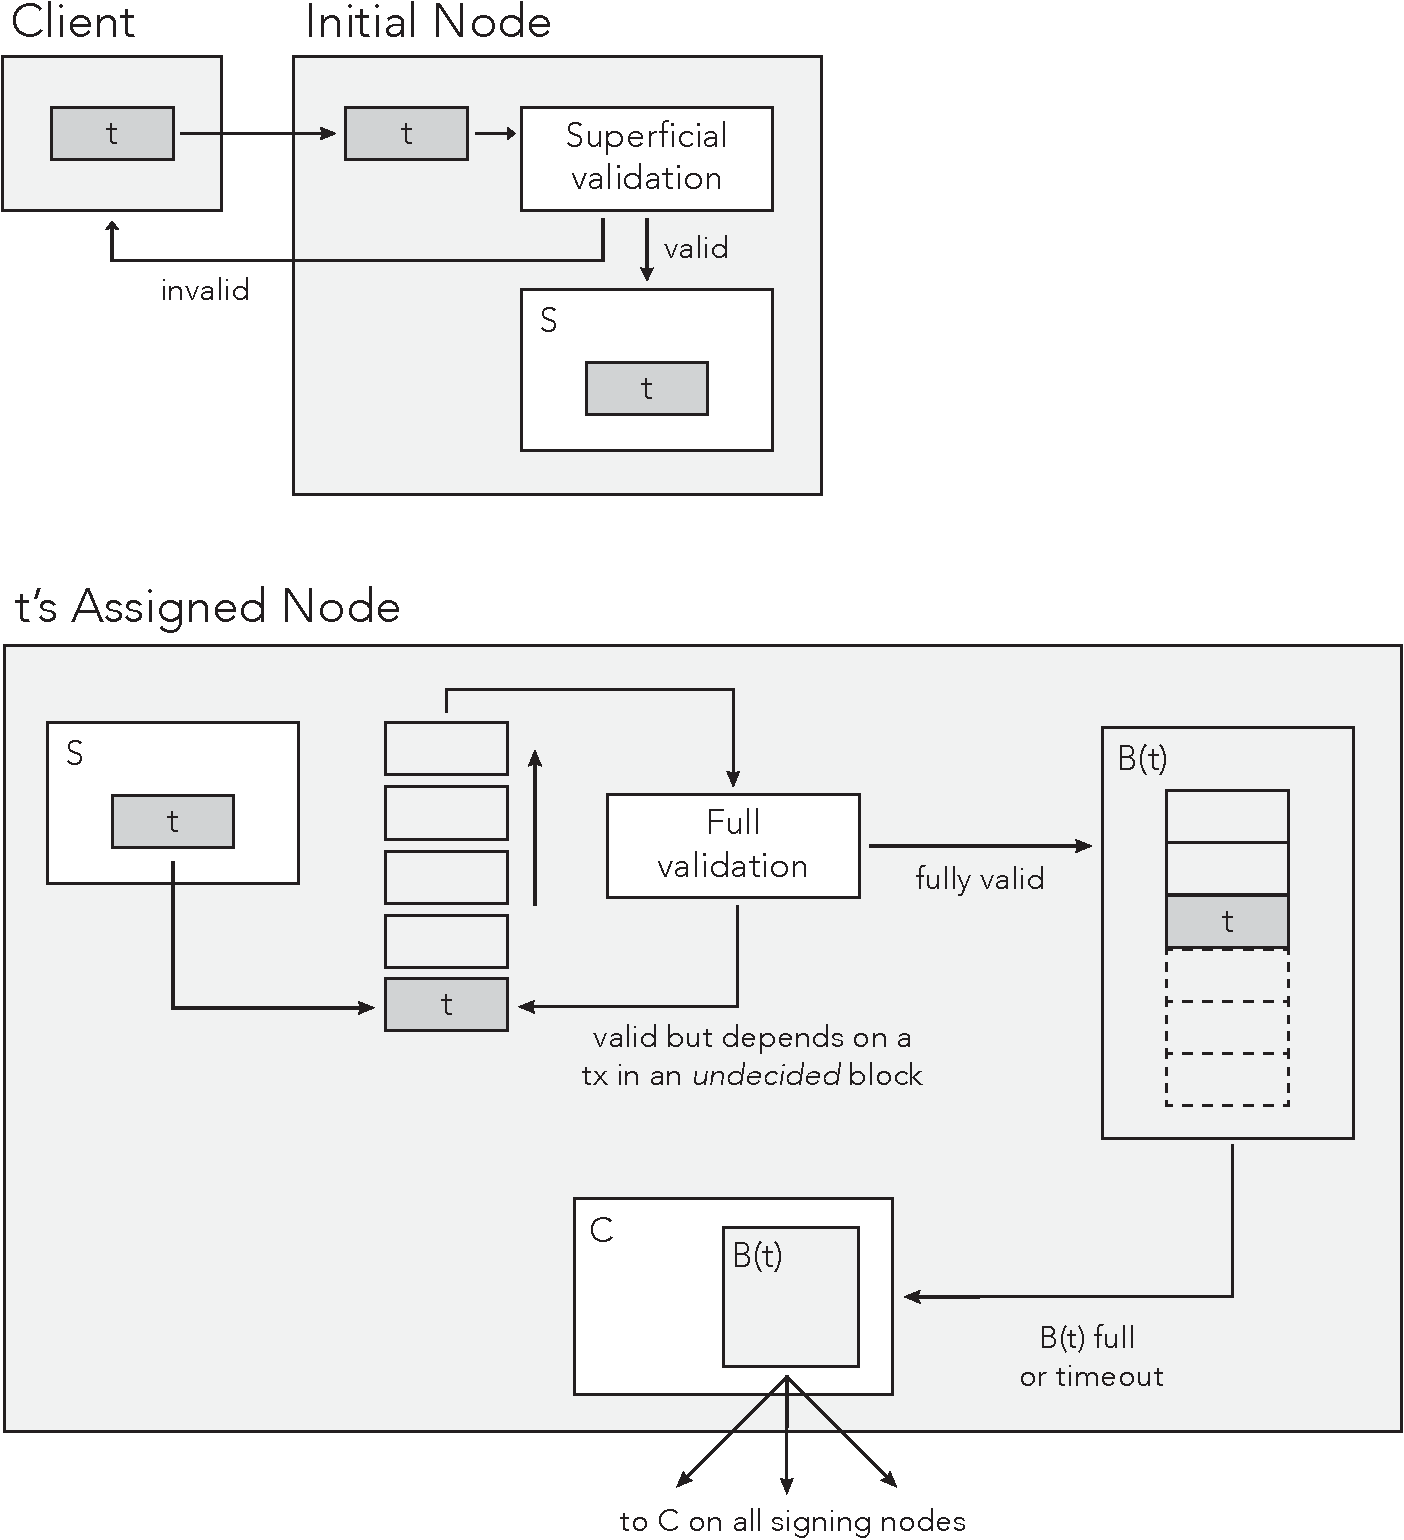
\includegraphics[width=0.8\textwidth]{figure_11.pdf}
  \caption{Life of a Transaction, Part 1/2}
  \label{fig:bigchaindb_tx_life_1}
\end{figure}

\begin{figure}[!ht]
  \centering
  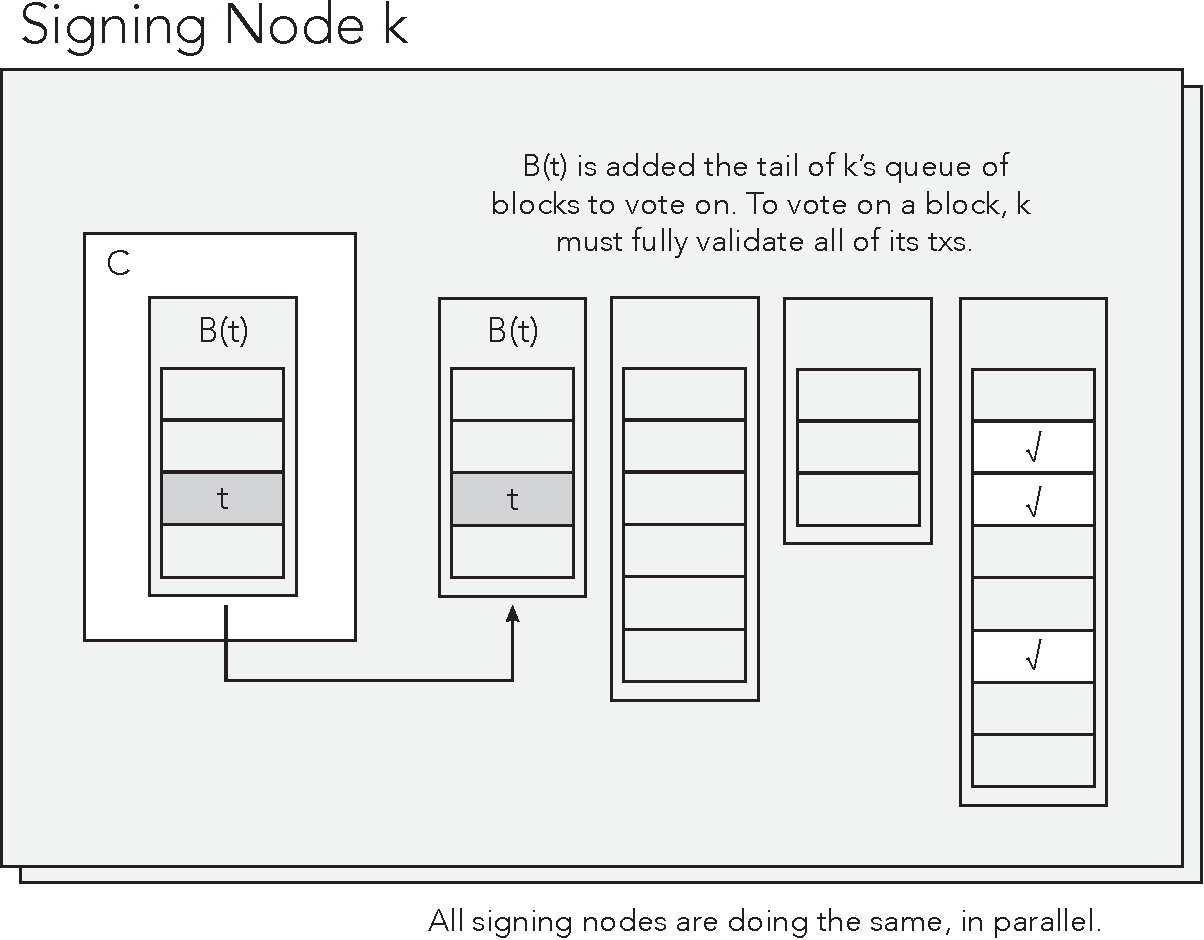
\includegraphics[width=0.6\textwidth]{figure_12.pdf}
  \caption{Life of a Transaction, Part 2/2}
  \label{fig:bigchaindb_tx_life_2}
\end{figure}

The time interval required for each step will vary. 
It can depend on how busy a node is, how busy the cluster is, network latency, and other factors. 
Nevertheless, we can still identify each step in the life of a transaction, to determine the main sources of latency.

Generally speaking, the client will send their transaction $\mathbf{t}$ over the Internet to a BigchainDB node. 
The transmission time $t_{\mathtt{in}}$ depends on how far the client is from the BigchainDB node, but it will typically range from tens to hundreds of milliseconds (ms). 
Once $\mathbf{t}$ is in a \textsf{\textit{decided\_valid}} block, a BigchainDB node can send a success notification to the client. 
The transmission time $t_{\mathtt{out}}$ will be approximately the same as $t_{\mathtt{in}}$. 
Figure \ref{fig:bigchaindb_tx_latency} illustrates $t_{\mathtt{in}}$ and $t_{\mathtt{out}}$.

We can write the total latency as:
\begin{equation}
  t_\mathtt{total} = t_{\mathtt{in}} + t_{\mathtt{internal}} + t_{\mathtt{out}}
\end{equation}

where $t_{\mathtt{internal}}$ is internal latency: the latency contributed by the Bigchain DB cluster itself. 
$t_{\mathtt{in}}$ and $t_{\mathtt{out}}$ depend on the client, but $t_{\mathtt{internal}}$ will be independent of the client (as a first approximation). 
The remainder of this section is focused on developing an estimate for $t_{\mathtt{internal}}$.

\begin{figure}[!ht]
  \centering
  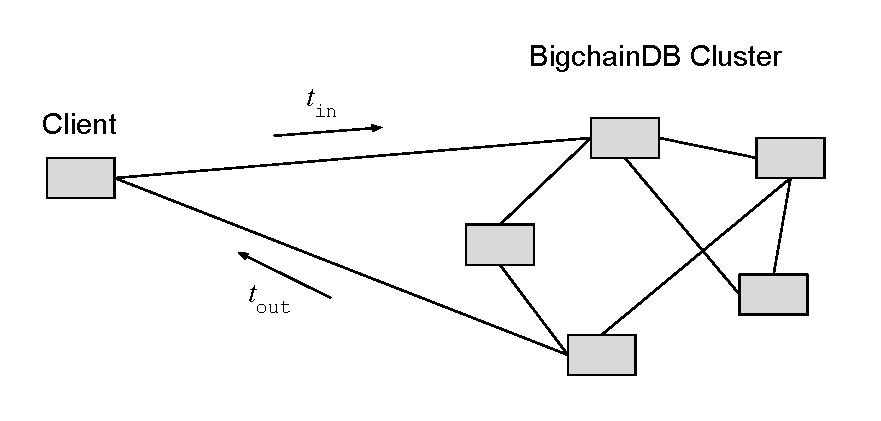
\includegraphics[width=0.7\textwidth]{figure_13.pdf}
  \caption{Transmission latencies between the client and the BigchainDB cluster.}
  \label{fig:bigchaindb_tx_latency}
\end{figure}

Let’s start with some notation.
There are many sources of latency within the BigchainDB cluster, but a key one is the time it takes information to travel from one node to another node. 
Let’s call the typical one-hop node-to-node latency $t_{\mathtt{hop}}$. The duration of $t_{\mathtt{hop}}$ depends a lot on how the nodes are distributed. 
If the nodes are all in one data center, then $t_{\mathtt{hop}}$ might be less than 1 ms. If the nodes are distributed globally, then $t_{\mathtt{hop}}$ might be $150$ ms.

Another key source of latency is query latency $t_{\mathtt{q}}$. 
If a node queries the underlying (distributed) database, it might happen that the node itself already has all the information it needs to determine the result. 
That is probably unusual. More typically, the required information is on one or more other nodes. 
Getting that information requires at least two internal network hops: one to send the query out, and one to get information back. 
For that case, we can write:
\begin{equation}\label{eq:time_query}
t_\mathtt{q} \le (2 \cdot t_\mathtt{hop}) + t_\mathtt{qp}
\end{equation}
where $t_\mathtt{qp}$ is the query processing time. 

If all nodes in the cluster are in one data center, then $t_\mathtt{hop}$ and $t_\mathtt{qp}$ might be similar in duration, so we may not be able to neglect $t_\mathtt{qp}$ relative to $t_\mathtt{hop}$.

Let’s return to figuring out a back-of-the-envelope estimate for $t_\mathtt{internal}$.
In general, it could be quite large, because a transaction might bounce back and forth between the backlog $\mathbf{S}$ and the bigchain $\mathbf{C}$ before it finally ends up in a \textsf{\textit{decided\_verified}} block.
What we \textit{can} do is determine an approximate \textit{minimum} $t_\mathtt{internal}$.

When $\mathbf{t}$ arrives at a BigchainDB node, the node does a superficial validation of $\mathbf{t}$ (i.e. not checking if it depends on a transaction in an undecided block). 
That requires at least one query (e.g. to check if $\mathbf{t}$ does a double-spend), so the time required is at least $t_\mathtt{q}$. 
(If $\mathbf{t}$ is invalid, then the client can be notified and that’s the end of the story for $\mathbf{t}$.)

If $\mathbf{t}$ is valid, then the BigchainDB node assigns $\mathbf{t}$ to a randomly-choosen node. 
It then writes $\mathbf{t}$ to the backlog ($\mathbf{S}$). 
The underlying distributed database will notify all the other nodes about the change to $\mathbf{S}$ (i.e. that there is a new transaction), along with the contents of $\mathbf{t}$. 
It takes at least $t_\mathtt{hop}$ time for $\mathbf{t}$ to propagate over the internal BigchainDB network.

$\mathbf{t}$ then enters the tail of a queue on the assigned node, where it waits for the assigned node to check it for validity (including whether $\mathbf{t}$ depends on a transaction in an \textsf{\textit{undecided}} block). 
In general, there may be several transactions ahead of $\mathbf{t}$ in that queue. 
The assigned node must check each of those transactions first; each check requires at least one query, so at least $t_\mathtt{q}$ time is needed to check each transaction ahead of $\mathbf{t}$. 
In the best case, there are no transactions ahead of $\mathbf{t}$ in the assigned node’s queue, so the waiting time is zero.

Once $\mathbf{t}$ gets its turn at being considered, the assigned node must check to see if $\mathbf{t}$ is valid (including whether $\mathbf{t}$ depends on a transaction in an \textsf{\textit{undecided}} block). 
That takes at least $t_\mathtt{q}$ time. 
If $\mathbf{t}$ \textit{does} depend on a transaction in an \textsf{\textit{undecided}} block, then it must go back to waiting for consideration for inclusion in a block (i.e. back to the tail of the assigned node’s queue).

Suppose $\mathbf{t}$ is okayed for inclusion in a block. 
Let’s call that block $\mathbf{B}(\mathbf{t})$. 
$\mathbf{t}$ must wait for $\mathbf{B}(\mathbf{t})$ to accumulate $1000$ transactions (or whatever value the BigchainDB operator sets), or for a timeout to occur (e.g. $5$ seconds since the last transaction was added to the block). 
The timeout is to ensure that a block doesn’t wait forever for new transactions. 
When there are lots of new transactions coming in, the time t spends waiting for $\mathbf{B}(\mathbf{t})$ to fill up will typically be negligible compared to $t_\mathtt{hop}$, so we can ignore it.

The assigned node then writes $\mathbf{B}(\mathbf{t})$ to $\mathbf{C}$. It takes time for $\mathbf{B}(\mathbf{t})$ to propagate to all other nodes in the cluster: at least $t_\mathtt{hop}$.

Each signing node will be notified about the new block $\mathbf{B}(\mathbf{t})$, including its contents. Signing node $\mathbf{k}$ will add the newly-arrived block to the tail of its queue of blocks to vote on. 
$\mathbf{k}$’s local copy of $\mathbf{B}(\mathbf{t})$ will wait for $\mathbf{k}$ to vote on all other blocks ahead of $\mathbf{B}(\mathbf{t})$ in $\mathbf{k}$’s queue. 
In the best case, there are no nodes ahead of $\mathbf{B}(\mathbf{t})$ in $\mathbf{k}$’s queue, so the waiting time is zero.

How long does it take for a node to vote on one block? 
If there are $1000$ transactions in the block, then the node may have to check the validity of all $1000$ transactions. 
(It doesn’t always have to check all the transactions: if it finds an invalid one, it can stop before checking any more.) 
Once the validity checks are done, the node must compose a vote (data structure) and calculate its digital signature, but the time to do that is negligible compared to the time needed to check validity.

The node doesn’t have to check the validity of each transaction one at a time. 
It can check many transactions in parallel at the same time, depending on how many processes are available to do validity-checking. 
In principle, there may be sufficient processors available to check all transactions for validity in parallel at once. 
Therefore, in the best case, the time to vote on one block will be approximately the same as the time to check one transaction for validity: $t_\mathtt{q}$.

Once $\mathbf{B}(\mathbf{t})$ gets to the head of $\mathbf{k}$’s queue, $\mathbf{B}(\mathbf{t})$ might already be decided, but $\mathbf{k}$ votes on it regardless (i.e. $\mathbf{k}$ doesn’t spend time checking if $\mathbf{B}(\mathbf{t})$ is already decided). 
As explained above, voting on $\mathbf{B}(\mathbf{t})$ takes at least $t_\mathtt{q}$ time.

Once $\mathbf{B}(\mathbf{t})$ has gotten votes from a majority of the signing nodes, it becomes either \textsf{\textit{decided\_valid}} or \textsf{\textit{decided\_invalid}}. 
(The list of nodes which can vote on $\mathbf{B}(\mathbf{t})$ is set when $\mathbf{B}(\mathbf{t})$ is created, and doesn’t change if nodes are added or removed from the cluster.) 
The deciding vote takes time $t_\mathtt{hop}$ to propagate to all the other nodes in the cluster.

If $\mathbf{B}(\mathbf{t})$ is \textsf{\textit{decided\_invalid}} then the transactions inside $\mathbf{B}(\mathbf{t})$ (including $\mathbf{t}$) get sent back to $\mathbf{S}$ for reconsideration in a future block.

If $\mathbf{B}(\mathbf{t})$ is \textsf{\textit{decided\_valid}}, then $\mathbf{t}$ is “etched in stone” and a success notification message can be sent to the client.

We can now estimate a minumum $t_\mathtt{internal}$ by adding up all the times outlined in the precedinging paragraphs:

\begin{equation}
 t_\mathtt{internal} \le 3 \cdot t_\mathtt{q} + 3 \cdot t_\mathtt{hop}
\end{equation}

Then, using eq. \eqref{eq:time_query}:

\begin{equation}
 t_\mathtt{internal} \le 9 \cdot t_\mathtt{hop} + 3 \cdot t_\mathtt{qp} 
\end{equation}

If the cluster nodes are widely-distributed, then $t_\mathtt{hop}$ is much larger than $t_\mathtt{qp}$ and:

\begin{equation}
 t_\mathtt{internal} \le 9 \cdot t_\mathtt{hop}
\end{equation}

As a rule of thumb for widely-distributed clusters, \textit{the minimum internal latency is about an order of magnitude larger than the one-hop node-to-node latency}. 
(Remember that $t_\mathtt{internal}$ ignores client-to-BigchainDB network latency.)

\begin{savenotes}
\begin{table}[ht!]
  \caption{Latency based on geography}
  \footnotesize
  \makebox[\textwidth][c]{
  \setlength\extrarowheight{3pt}
  \begin{tabular}{ | m{\dimexpr 0.3\linewidth-2\tabcolsep} |
	  M{\dimexpr 0.35\linewidth-2\tabcolsep} |
	  M{\dimexpr 0.35\linewidth-2\tabcolsep} |} \Xhline{4\arrayrulewidth}\rowcolor{black}
    \color{white}How nodes are distributed    &  \color{white} One-hop node-to-node latency in the cluster ($t_\mathtt{hop}$) & \color{white} Cluster internal transaction latency ($t_\mathtt{internal}$) \\\Xhline{4\arrayrulewidth}
    In one data center           & $\approx 0.25$ ms & $\le 2.25$ ms\footnote{This estimate doesn’t include the query-processing term ($3 \cdot t_\mathtt{qp}$), which might be about the same magnitude (i.e. milliseconds).} \\\hline
    In one region (e.g. America) & $\approx 70$ ms   & $\le 630$ ms \\\hline
    Spread globally              & $\approx 150$ ms  & $\le 1350$ ms \\
  \Xhline{4\arrayrulewidth}
  \end{tabular}
  }
  \label{tab:latency_comparison}
\end{table}
\end{savenotes}

There are a few general cases, depending on how the BigchainDB nodes are distributed. Table \ref{tab:latency_comparison} summarizes.

The latency estimates in Table \ref{tab:latency_comparison} are order-of-magnitude approximations. They can be interpreted as guidelines for what to expect.